\chapter{Introduction}

\label{chapter:intro}

Micro unmanned aerial vehicles (MAVs, also called drones) recently saw a rise in usage across various fields. 
Drones are already widely used in cinematography \cite{Mademlis2020}, advertising \cite{Ullah2021} and agriculture \cite{Kim2019}. 
City emergency departments also use Unmanned Arial Vehicles (UAVs) - firefighters can use them to see and evaluate the situation from the sky, localize the source of fire and put it out \cite{Pritzl2021}.
Another field where MAVs can be used in nearest future is transportation. 
Fast parcel delivery \cite{She2021} and content transportastions \cite{Gupta2021,Aloqaily2022} are quite promissing fields of UAV application together with smart city concepts evolving \cite{Ortiz2019}.
Nowadays, even collaborative transportation systems are becoming realistic - multi-robot swarming algorithms are better developed, and that allows their usage for the transportation of large objects \cite{Bacelar2020} that one drone can not lift. 
MAVs are also widely used in the military industry.

As drones are used so widely, there is a large demand for an increas in drone-related safety. 
Many commercially available drones are expensive and quite heavy, so accidents can be costly and dangerous to property and human health. 
Even if a drone is on remote control, when the pilot flies on a long distance, obstacles can be hard to spot and avoid.
Same about flying in a forest or in cities (in situations when it is legal, for example - emergency departments and movie makers can do it), obstacles can not be observed.
In such situations, the best for the pilot would be to use first person view glasses, which provides the field of view (FOV) not bigger than FOV of human's eyes (which is about $130^\circ$), but dangerous obstacles can appear from any side.
In this sence, autonomous robots can see and avoid obstacles much better, but only if they have a well-designed system running onboard and enough sensors to cover the area around a drone.

Automatic obstacle avoidance systems become especially important in closed environments with many obstacles, such as a forest, a city, or indoor environments.
To ensure a full coverage of the surroundings of the MAV for the collision avoidance system, it can be equipped with multiple sensors pointing in all directions.

Considering this context above, a compact obstacle avoidance system is a perspective field for research. 
Even though the idea is not new, neither DJI, MRS, nor other research groups have a well-developed visual obstacle avoidance system. 
The best, for now, can be the Skydio system\footnote{\href{https://www.skydio.com/skydio-autonomy}{Skydio autonomy: https://www.skydio.com/skydio-autonomy }}, but their approach is for a forward-moving drone.

The inspiration for this project was taken from DJI's obstacle avoidance technology introduced with the release of the DJI Mavic 3 drone\footnote{\href{https://www.dji.com/cz/mavic-3}{DJI Mavic 3: https://www.dji.com/cz/mavic-3}}. 
It uses visual data from monocular cameras with overlapping fields of view to cover almost the whole area around the UAV and react in real-time to obstacles nearby. 
Unfortunately, they have no publications or implementation details, so it is only a conclusion from publicly available information.

\begin{figure}[t]
    \centering
    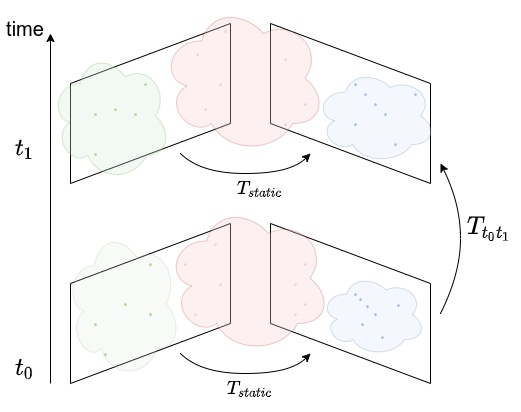
\includegraphics[width=0.6\textwidth]{graphics/general_scheme.png}
    \caption{ A general scheme of the multi-camera obstacle detection problem.}
    \label{fig:intro_general}
\end{figure}

\autoref{fig:intro_general} presents a scheme of the proposed system.
In the figure, $T_{static}$ is the transformation between two cameras onboard the MAV obtained with stereo pair calibration. 
At time $t_0$, a new pair of images is captured by the cameras.
A feature detector extracts points of interest from the image.
Points that lie in the part of the images corresponding to a section of the cameras' field of view that overlaps (the red point cloud in \autoref{fig:intro_general}) are then selected and correspondence matches between these points from the two images are found based on their features.
A calibrated projection model of the cameras and the transformation $T_{static}$ are used to estimate 3D points from the matched point pairs.
Then at time $t_1$, when a new pair of images is received, the same process is repeated. 
In parallel, an incremental Structure from Motion (SfM) algorithm processes sequences of images from each camera separately to estimate 3D points, corresponding to nearby objects in the environment. However, monocular SfM algorithms can generally only estimate the environment up to an unknown scaling factor \cite{SfM}. To address this problem, the red point cloud is used to find the scale of the points obtained using the SfM algorithm from images captured at $t_0$ and $t_1$ (the blue and green point clouds in \autoref{fig:intro_general}).

\section{Related Works}
Various MAVs use several obstacle avoidance sensors: stereo vision \cite{Ruf2018}, depth cameras (as Intel RealSense), monocular vision \cite{Mejias2010}, lidar (2d or 3d) \cite{Ramasamy2016}, sonar (ultrasonic), time of flight sensors, also combinations of them can be used. 

Each of them has its pros and cons. 
3D lidars are more expensive than other sensors, but they can provide good accuracy, precision and 3d coverage of the environment; 2d lidars are successfully used for ground vehicles, but they are not so suitable for most tasks for MAVs because a car can be modelled as 2 degrees of freedom (DoF) system, while MAVs always have 4DoF, some specialized even up to 6DoF. 
Depth cameras are more expensive than simple cameras. Ultrasonic and infrared sensors have distance limits and other minor issues ( a.e. sonar can be influenced by noise from the MAVs). 

In most articles, a stereo pair of two parallel cameras looking in the same direction (classical stereo pair) \cite{Lin2021} is used.
Deep learning approaches \cite{Back2020, FragaLamas2019, Park2020, Roghair2021} and Convolutional Neural Networks \cite{Yu2013, Ma2020} are also quite popular.
A real-time multi-camera feedback control system that considers several cameras placed on multiple drones is introduced in \cite{He2021}.

Real-time simultaneous localization and mapping (SLAM) systems can also be used for obstacle avoidance \cite{Moreno2014}. 
These problems are pretty closely related. 
SLAM keeps track of the robot's position while constructing and updating a map of an unknown environment, while obstacle avoidance is a problem of detecting and avoiding the nearest obstacles in an unknown environment to keep the robot safe from harmful collisions.
Both problems are related to making a 3D map of an unknown environment, but for obstacle avoidance, the precision of distance measurements to the nearest objects is much more critical.

\begin{figure}[h]
    \begin{subfigure}[h]{0.31\textwidth}
      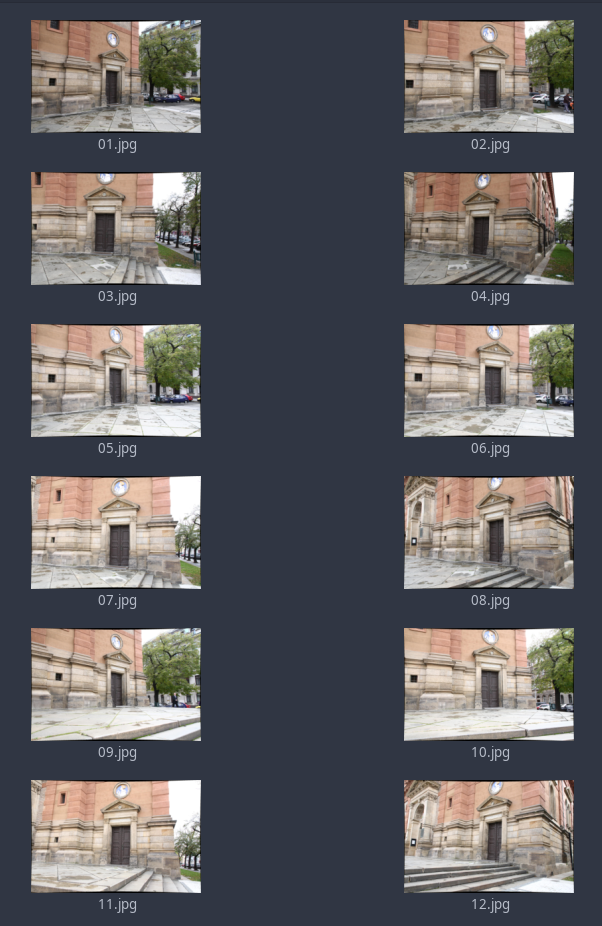
\includegraphics[width=\textwidth]{graphics/input_set.png}
      \caption{Input images.}
      \label{fig:pc_input}
    \end{subfigure}
    \hfill
    \begin{subfigure}[h]{0.65\textwidth}
      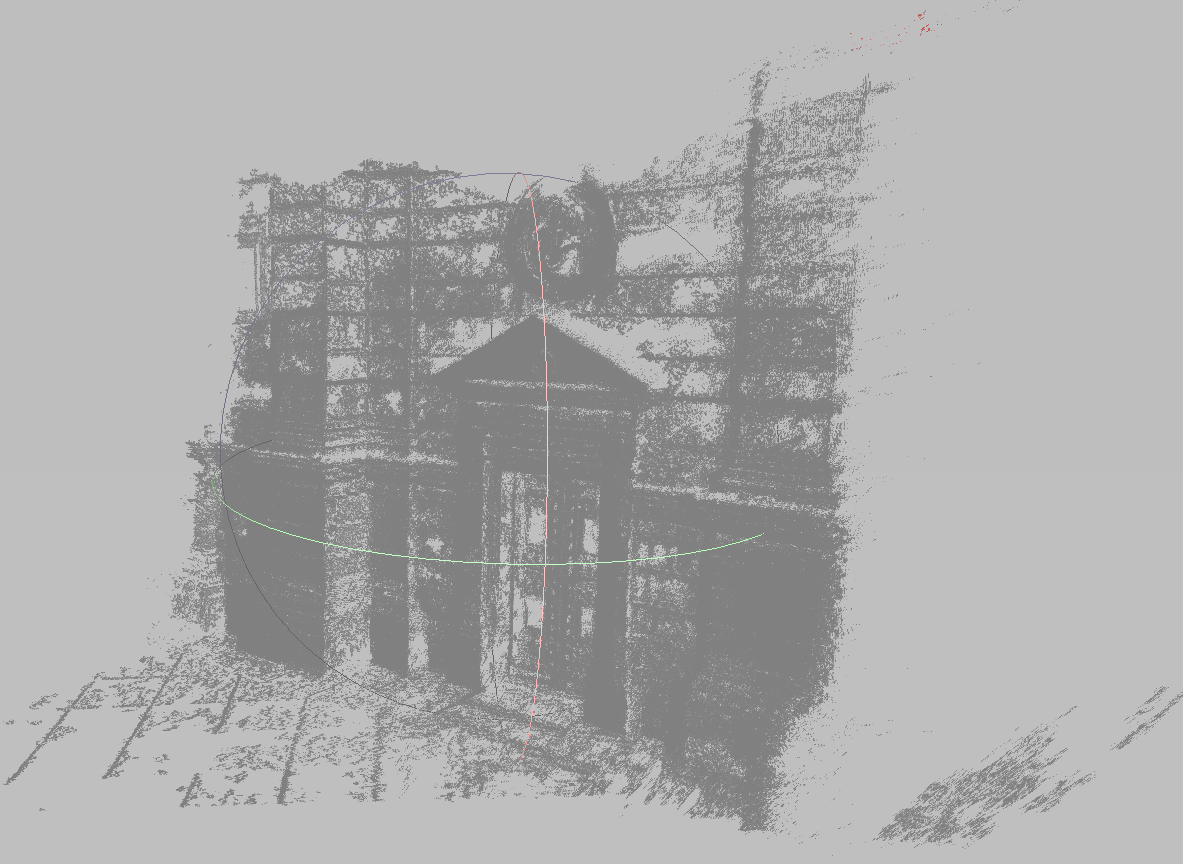
\includegraphics[width=\textwidth]{graphics/reconstructed.png}
      \caption{Output of an SfM algorithm.}
      \label{fig:pc_output}
    \end{subfigure}
    \caption[Ilustration of Structure from Motion.]{Ilustration of Structure from Motion, source - \url{https://github.com/Myralllka/CTU_3d_computer_vision/}}
    \label{fig:pc_recons}
\end{figure}

Structure from Motion (SfM) is another family of algorithms that may be used to implement a system for avoiding obstacles. 
SfM is a method of depth map reconstruction from a continuous sequence of images as in the \autoref{fig:pc_input}.
Using this approach, a dense point cloud as in \autoref{fig:pc_output} can be computed and obstacles can be detected \cite{Lee2008}. 

\section{Problem definition}
\label{sec:problem_definition}
This thesis aims to design a visual obstacle avoidance system for MAVs, create a physical device implementing the system and measure its performance. 
The proposed solution assumes an MAV with a limited size and lifting force that constraints the number, weight and size of its onboard sensory equipment. 
The MAV is thus equipped with two calibrated cameras with a known transformation between them. 
The fields of view of the cameras overlap enough to detect close obstacles.
Framerate of the cameras is sufficient to operate in real-time (at least 30 frames per second (fps)), and the frames are synchronized in time.
The MAV is also equipped with an onboard computer with enough computational power to process the images at a rate sufficient for the obstacle avoidance.
The flight environment is assumed to be well-lit and to contain objects with well-distinguishable visual features that the cameras can observe.
These features should be unique so that the same feature can be unambiguously matched in images from the two cameras.
The expected output is a reconstruction of the 3D environment around the drone in the form of a set of points representing the nearest objects.
Depending on the estimated distance, these are the possible obstacles that should be avoided.
The system can be integrated with the MAV control system to provide it with obstacles, so the solution working rate on the MAV's hardware should be sufficient enough for agile manoeuvering and obstacle avoidance.

